\documentclass[../main.tex]{subfiles}

\begin{document}

In questa sezione ricavo l'equazione del moto perturbato che descrive i modi normali del Sole: considero piccole perturbazioni dello stato di equilibrio e adiabatiche cio\'e molto pi\'u rapide del tempo scala per scambio di calore dovuto al flusso radiativo o alle reazioni nucleari. Le frequenze delle oscillazioni adiabatiche sono determinate dalla struttura interna del Sole attraverso i coefficienti che compaiono nelle equazioni che descrivono i modi normali: dato che $P,\ \rho,\ g$ non sono indipendenti \'e sufficiente specificare $\rho(r)$ e $\Gamma_1(r)$. Un confronto con le frequenze osservate necessita che la precisione numerica sia dei parametri ricavati dal modello sia delle tecniche numeriche usate per ricavare le frequenze dei modi di oscillazione sia maggiore dell'accuratezza delle misure.


{\let\clearpage\relax
\chapter{Perturbazioni lineari adiabatiche.}
}

\begingroup
\color{midnightblue}


\subsection{Onde stazionarie: modo fondamentale.}

Le oscillazioni solari sono in prevalenza dovute ad onde acustiche, in cui la forza di richiamo \'e prodotta dal gradiente di pressione: il profilo radiale della velocit\'a del suono determina il loro comportamento all'interno del Sole.

I modi puramente acustici di un corpo finito o comunque con condizioni ai bordi sono onde stazionarie la cui parte reale \'e del tipo $f(x,y,z)\cos{(\omega t+\alpha)}$: in assenza di effetti dissipativi la velocit\'a di fase \'e nulla e la velocit\'a di gruppo infinita, velocit\'a e pressione sono sfasati di $\frac{\pi}{2}$. 

Per un corpo in equilibrio idrostatico ricavo il valore medio della velocit\'a del suono utilizzando il teorema del viriale
\begin{align}
&-\Omega=3\int_VP\,dV=3\int_M\frac{P}{\rho}\,dm=3\int_M\frac{c_s^2}{\Gamma_1}\,dm=3\exv{\frac{c_s^2}{\Gamma_1}}M\approx3\frac{\overline{c}_s^2}{\Gamma_1}M
\end{align}

Per stelle in sequenza principale ho $\Omega=-q\frac{GM^2}{R}$ con $q\approx1.5$; per il modo fondamentale di oscillazione radiale si ha:
\begin{align*}
 &\lambda_1\approx 2\rsun{},\ \omega_1\approx\frac{c_s}{\lambda_1},\ \Pi_1\approx\SI{1}{\hour}
\end{align*}

\endgroup

\section{Perturbazione dello stato di equilibrio.}


Descrivo le oscillazioni come piccole perturbazioni attorno allo stato di equilibrio stazionario (gli effetti non lineari sono dell'ordine di $\frac{v}{c_s}$ dove v \'e l'ampiezza dell'oscillazione). Indico con $P'(\vec{r},t)$ la perturbazione euleriana, con $\delta\vec{r}=\vec{\xi}$ lo spostamento della particella di fluido a causa della perturbazione e con $\vec{v}=\PDof{t}(\Lvar{\vec{\xi}})$ la sua  velocit\'a

\begin{equation}
P(\vec{r},t)=P_0(\vec{r})+P'(\vec{r},t)\label{eq:pressureperturbation}
\end{equation}

e in termini della variazione lagrangiana

\begin{equation*}
\Lvar{P(\vec{r})}=P(\vec{r}+\Lvar{\vec{r}})-P_0(\vec{r})=P'(\vec{r})+\Lvar{\vec{r}}\cdot\nabla P_0
\end{equation*}



Ricavo l'equazione del moto perturbato sostituendo \eqref{eq:pressureperturbation} nell'equazione del moto  $\rho\TDof{t}v\indices{_i}=\rho(\PDy{t}{v\indices{_i}}+v\indices{_j}\partial\indices{_j}v\indices{_i})=-\partial\indices{_i} P+\rho\vec{g}\indices{_i}$ e considerando solo i termini lineari nelle perturbazioni risulta:

\begin{equation}
\rho_0\PtwoDy{t}{\Lvar{\vec{r}}}=\rho_0\PDy{t}{\vec{v}}=-\nabla P'+\rho_0\vec{g}'+\rho'\vec{g}_0\label{eq:emper}
\end{equation}

con $\vec{g}'=-\nabla\Phi'$, $\nabla^2\Phi'=4\pi G\rho'$.

Analogamente per l'equazione di continuit\'a ottengo
\begin{equation}
\rho'+\div{(\rho_0\Lvar{\vec{r}})}=0\label{eq:contper}
\end{equation}


\subsection{Approssimazione adiabatica.}

I tempi caratteristici per scambio di calore sono molto maggiori del periodo delle pulsazioni. Considero i termini a destra dell'equazione di conservazione dell'energia interna \eqref{eq:primatemp}, dove ho esplicitato il bilancio di calore usando \eqref{eq:heatgl},


\begin{equation*}
\TDy{t}{T}-\frac{\Gamma_2-1}{\Gamma_2}\frac{T}{P}\TDy{t}{P}=\frac{1}{c_P}(\epsilon-\frac{1}{\rho}\scap{\nabla}{F})
\end{equation*}

Stimo il tempo caratteristico $\tau_R$ per flusso radiativo \eqref{eq:radfluxTgradrelation}:

\begin{align*}
&\frac{1}{\rho c_P}\nabla\cdot(\frac{4acT^3}{3\kappa\rho}\nabla T)\approx\frac{4acT^4}{3\kappa\rho^2c_PH}=\frac{T}{\tau_R}&\intertext{H lunghezza caratteristica, in cgs:}\\
&\tau_R=\num{e12}\frac{\kappa\rho^2H^2}{T^3}
\end{align*}

Per valori caratteristici dell'intero Sole ho ($\kappa=1$, $\rho=1$, $T=\num{e6}$, $H=\num{e10}$) ho $\tau_R\approx\SI{e7}{\year}\approx\tkh{}$, per valori caratteristici della zona convettiva ($\kappa=100$, $\rho=\num{e-5}$, $T=\num{e4}$, $H=\num{e9}$) ho $\tau_R\approx\SI{e3}{\year}$, in cgs.


Nella parte interna il termine dovuto alle reazioni nucleari \'e caratterizzato da un tempo $\tau_{\epsilon}\approx\frac{c_PT}{\epsilon}\approx\tkh{}$.

Confronto $\frac{T}{\tau_R}$, $\frac{T}{\tau_{\epsilon}}$ con $\TDy{t}{T}\approx\frac{T}{\Pi_{osc}}$ con $\Pi_{osc}\approx\si{\minute}-\si{\hour}$: i termini dovuti allo scambio di calore sono trascurabili rispetto alla derivata temporale di T.

Il moto di una elemento di fluido \'e descritto dalla relazione adiabatica


\begin{align*}
&\TDy{t}{P}=\frac{\Gamma_1P}{\rho}\TDy{t}{\rho}
\end{align*}

Approssimazione adiabatica non pi\'u valida vicino alla superficie solare dove i tempi per lo scambio di calore sono pi\'u brevi.

La condizione di perturbazione adiabatica linearizzata \'e
\begin{align}
&\PDy{t}{\Lvar{P}}-\frac{\Gamma_{1,0}P_0}{\rho_0}\PDy{t}{\Lvar{\rho}}=0\nonumber&\intertext{che integrata rispetto a t ed in funzione della variazione euleriana diventa}\nonumber\\
&P'+\Lvar{\vec{\xi}}\cdot\nabla P_0=\frac{\Gamma_{1,0}P_0}{\rho}(\rho'+\Lvar{\vec{\xi}}\cdot\nabla\rho_0)\label{eq:adper}
\end{align}

\section{Modi di oscillazione.}

\subsection{Separazione variabili spaziali e temporali.}

Dall'equazione del moto \eqref{eq:emper} si vede che

\begin{equation*}
\hat{r}\cdot(\rot{\PtwoDy{t}{\vec{\xi}}})=0\ \Rightarrow\ \PDof{\theta}(\sin{\theta}\xi_{\phi})-\PDy{\phi}{\xi_{\theta}}=0
\end{equation*}

quindi \'e possibile ricavare la componente tangenziale della perturbazione da una funzione scalare.

Descrivo i modi normali di oscillazione introducendo la dipendenza temporale da $\exp{i\omega t}$ e angolare dalle funzioni armoniche sferiche $Y_{lm}(\theta,\phi)$

\begin{equation}
\vec{\xi}=\exp{i\omega t}(\xi_r(r),\xi_h(r)\PDof{\theta},\frac{\xi_h(r)}{\sin{\theta}}\PDof{\phi})Y_l^m(\theta,\phi)
\end{equation}

dove ho scomposto il vettore spostamento perturbato in componente radiale $\xi_r(r)$ e tangenziale $\xi_h(r)$.

Le funzioni armoniche sferiche  soddisfano
\begin{equation}
L^2Y_l^m=-\frac{1}{\sin{\theta}}\PDof{\theta}(\sin{\theta}\PDy{\theta}{Y_l^m})+\frac{1}{\sin^2{\theta}}\PtwoDy{\phi}{Y_l^m}=-r^2\nabla_h^2Y_l^m=l(l+1)Y_l^m\label{eq:SHperturb}
\end{equation}

La variazione euleriana di densit\'a, pressione, potenziale gravitazionale sono espresse
\begin{align*}
&(\rho',P',\Phi')=\exp{i\omega t}[\rho'(r),P'(r),\Phi'(r)]Y_l^m
\end{align*}


\subsection{Spettro delle oscillazioni.}

Utilizzo l'equzione del moto \eqref{eq:emper} e l'equazione di continuit\'a \eqref{eq:contper} per eliminare $\xi_h(r)$ dall'equazione del moto
\begin{align}
&\frac{1}{r^2}\TDof{r}(r^2\xi_r)-\frac{\xi_rg}{c^2}+\frac{1}{\rho_0}(\frac{1}{c^2}-\frac{l(l+1)}{r^2\omega^2})P'-\frac{l(l+1)}{r^2\omega^2}\Phi'=0\nonumber\\
&\frac{1}{\rho_0}(\TDof{r}+\frac{g}{c^2})P'-(\omega^2-N^2)\xi_r+\TDy{r}{\Phi'}=0\label{eq:eigenomega}\\
&\frac{1}{r^2}\TDof{r}(r^2\TDy{r}{\Phi'})-\frac{l(l+1)}{r^2}\Phi'-\frac{4\pi G\rho_0}{g}N^2\xi_r-\frac{4\pi G}{c^2}P'=0\nonumber
\end{align}

con $g=-\frac{1}{\rho_0}\TDy{r}{P_0},\ c^2=\frac{\Gamma_1P_0}{\rho_0}$ e le frequenze critiche sono definite ho nella sezione \ref{sec:resonantcavity}.


Il sistema di equazione \eqref{eq:eigenomega} ha soluzione con le opportune equazioni al contorno per un insieme discreto di valori delle frequenze, $\omega_{nlm}$. L'ordine angolare non compare nelle equazioni quindi gli autovalori $\omega_{nlm}$ sono $2l+1$ degeneri: la degenerazione \'e rimossa nel caso si tenga conto della rotazione ($\frac{\Omega}{\omega}\approx\num{e-4}$) o di effetti gravitazionali di altri corpi.


Condizioni al contorno: sono necessarie 4 condizioni.

\begin{itemize}
\item Due condizioni per $r=0$ selezionano le soluzioni regolari:

\begin{equation}
P'=0,\ \Phi'=0
\end{equation}

Vicino a zero risulta un andamento asintotico

\begin{align*}
&(l\neq0):\ \xi_r\propto r\expy{l-1};\ (l=0):\ \xi_r\propto r\\
&P',\ \Phi'\propto r^l
\end{align*}

\item Alla superficie solare richiediamo la continuit\'a di $\Lvar{\nabla\Phi}$ e che non si abbia propagazione verso l'esterno.

All'esterno della stella ho $\rho'=0$ quindi scelgo la soluzione nulla a infinito dell'equazione di Poisson $\Phi'=Ar\expy{-l-1}$:

\begin{equation}
\TDy{r}{\Phi'}+\frac{l+1}{r}\Phi'=0,\ r=\rsun{}    
\end{equation}

La condizione di non propagazione oltre la fotosfera dipende dalla descrizione dell'atmosfera solare. Nella versione pi\'u semplice impongo che la variazione di pressione sia zero alla superficie perturbata della stella

\begin{align}
&\Lvar{P}=P'+\xi_r\TDy{r}{P}=0
\end{align}

\end{itemize}

[Fig.3 pag. 13 \cite{chr02helioseismology}]


\section{Eccitazione e tempo di vita dei modi.}

La presenza di modi osservabili pone il problema del bilancio energetico dei modi: si deve capire se esistono modi instabili, cio\'e modi per cui l'ampiezza delle oscillazioni lineari cresce


[Si ipotizza che le oscillazioni siano eccitate in maniera stocastica dai moti convettivi: la larghezza delle frequenze risonanti \'e determinata dal tempo di smorzamento.]

[Thermal over-stability: ulrich70, stein leibacher71]

[Extensive turbolent layers: stars lose all hint of vibrational instability]

[Not self excited: driven to observable amplitude by external process]

[Turbolent convection: source of pulsational energy, emit acustic radiation]

[Stable pulsation: spectrum as that of an ensemble of harmonic oscillator stocastically driven and damped]

[Power spectrum indipendent of l for $l<100$: low degree modes are not influenced by $k_h$. Vertical propagation: superficial layers (low l modes are generated in these strata)]

[Oscillations are intrinsically over-stable?]

[Interaction with turbolent convection]

[Radiative transfer (as frequencies rise modes became more sensitive to rapid relaxation time in solar atmosphere)]

[La stabilit\'a dei modi g \'e determinata dalla stabilit\'a convettiva: se non sono presenti regioni di instabilit\'a convettiva i modi g sono stabili ($g_+$), se esistono zone convettivamente instabili esistono anche modi g instabili ($g_{\,-}$).]

[Excitation p-modes: fluctuating turbolent pressure (Raynold stresses). Excitation g-modes: nuclear burning instabilities. Damping: radiative losses, viscosity, nonlinear interaction between modes.]

[Low l p-modes exponential decay with e-folding time several days.]


{\let\clearpage\relax           %%% Chapter  Caratteristiche asintotiche delle oscillazioni adiabatiche.
\chapter{Caratteristiche asintotiche delle oscillazioni adiabatiche.}\label{chap:asyntoticbehavour}
}

%[inserisci figura propagation ag]

I modi gravo-acustici descritti in \eqref{eq:eigenomega} si riducono ai modi p ed f per alte frequenze e ai modi g per basse frequenze. Approssimando il comportamento della perturbazione localmente con un'onda piana e trascurando la perturbazione al potenziale gravitazionale $\Phi'$ si ottendono soluzioni asintotiche per gli autovettori e le frequenze dei modi normali.

\section{Comportamento asintotico.}

Per determinare la struttura dello spettro delle oscillazioni introduciamo l'approssimazione di Cowling (\cite{cow41oscillations}) cio\'e trascuriamo la perturbazione del potenziale gravitazionale. Quindi il sistema \eqref{eq:eigenomega} si riduce al secondo ordine

\begin{align}
&\frac{1}{r^2}\TDof{r}(r^2\xi_r)-\frac{\xi_rg}{c^2}+\frac{1}{\rho_0}(\frac{1}{c^2}-\frac{l(l+1)}{r^2\omega^2})P'=0\label{eq:cowosc}\\
&\frac{1}{\rho_0}(\TDof{r}+\frac{g}{c^2})P'-(\omega^2-N^2)\xi_r=0\nonumber
\end{align}

Considero i limiti asintotici di alte e basse frequenze: ottengo un problema del tipo di Sturm-Liuville.
%https://en.wikipedia.org/wiki/Sturm%E2%80%93Liouville_theory

\begin{itemize}
\item Per $\omega\to\infty$:

Lo spettro \'e discreto, le oscillazioni sono prodotte da onde acustiche in cui la forza dominante \'e fornita dalla pressione, i modi p, ordinati in base al numero di zeri di $\xi_r$ fra il centro e la superficie.

\item Per $\omega\to0$:

Lo spettro \'e discreto, il moto \'e determinato dalla forza di gravit\'a, ho i modi g, ordinati secondo il numero di nodi radiali.

\end{itemize}

Lo spettro solare \'e la combinazione dei modi parziali precedenti; i modi f separano i modi g e p: non hanno nodi in direzione radiale.

{\itshape Relazione di dispersione per i modi gravo-acustici.}

Approssimo il comportamento spaziale delle oscillazioni con quello di onda piana
\begin{align*}
&\vec{\xi}\propto\exp{i\scap{k}{x}},\ \vec{k}=k_r\hat{r}+\vec{k}_h\\
&S_l^2=\frac{l(l+1)c^2}{r^2}\approx k_h^2c^2
\end{align*}

Considero i coefficienti delle equazioni \eqref{eq:cowosc} costanti ad eccezione di $P_0,\ \rho_0$: approssimazione valida se la lunghezza d'onda delle perturbazioni \'e molto minore della scala caratteristica di variazione dei coefficienti.

%stix local treatment pg 165


Sostituisco
\begin{align}
&\xi_r\propto\rho_0\expy{-\frac{1}{2}}\exp{ik_rr},\ P_1\propto\rho_0\expy{\frac{1}{2}}\exp{ik_rr}\&\intertext{forma richiesta dalla conservazione dell'energia e della quantit\'a di moto, e ottengo la relazione di dispersione:}\nonumber\\
&k_r^2=\frac{\omega^2-\omega_A^2}{c^2}+S_l\frac{N^2-\omega^2}{c^2\omega^2}=\frac{\omega^2}{c^2}(1-\frac{\omega_{l,+}^2}{\omega^2})(1-\frac{\omega_{l,-}^2}{\omega^2})\label{eq:localdispersion}&\intertext{e quindi determino le frequenze critiche per i modi gravo-acustici}\nonumber\\
&\omega_{\pm}=\frac{1}{2}(S_l^2+\omega_c^2)\pm\sqrt{\frac{1}{2}(S_l^2+\omega_c^2)^2-N^2S_l^2}
\end{align}

I modi di oscillazione soddisfano la relazione
\begin{equation}
\omega\int_{r_1}^{r_2}\sqrt{1-\frac{\omega_c^2}{\omega^2}-\frac{S_l^2}{\omega^2}(1-\frac{N^2}{\omega^2})}\,\frac{dr}{c}\approx\pi(n-\frac{1}{2})\label{eq:JWKBmode}
\end{equation}

\section{Cavit\'a risonanti.} \label{sec:resonantcavity} %Definizione frequenze critiche

La parte superiore dello spettro delle oscillazioni \'e caratterizzata da modi acustici mentre la parte inferiore \'e caratterizzata da modi di gravit\'a (vedere capitolo \ref{chap:asyntoticbehavour}). La variazione delle propriet\'a del gas influenzano la velocit\'a del suono, $c_s=\Gamma_1\frac{P}{\rho}$, e le frequenze critiche: esistono regioni dell'interno solare, dipendenti dalla natura delle oscillazioni, in cui \'e possibile un comportamento periodico ai cui bordi si ha riflessione interna.

\begin{minipage}{\linewidth}
\begin{tikzpicture}
\node[inner sep=0pt] (image) at (-0.5,0)
  {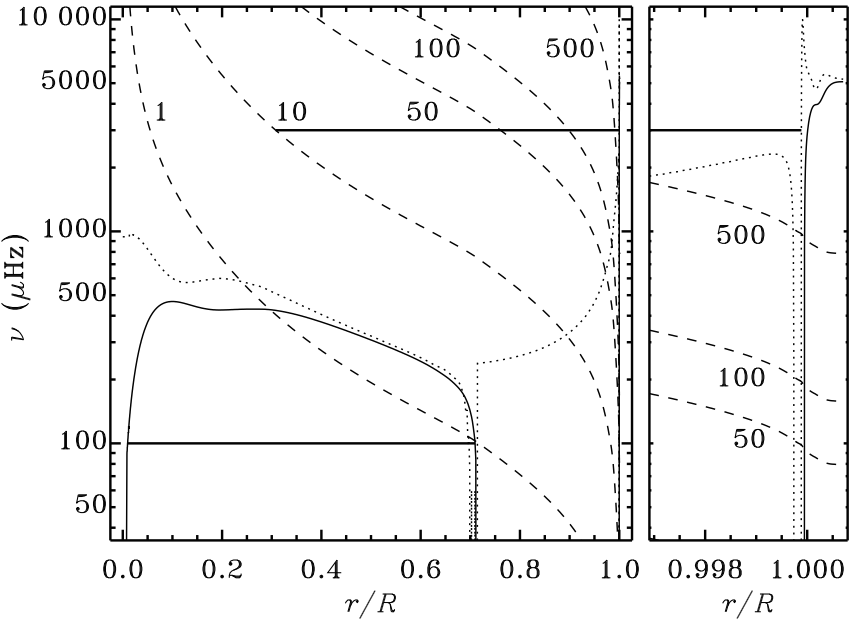
\includegraphics[keepaspectratio=true,scale=0.35]{cutoff}};
  \node (legenda) at (5.8,3) { Legenda };
  \draw [draw=black!50] (legenda.north west) rectangle +(0.35\textwidth, -4cm);
  \draw [dotted] (6,2) -- (5.5,2) node[at start, anchor=west] {$\frac{\omega_c}{2\pi}$;};
  \draw [dashed] (7.5,2) -- (7,2) node[at start, anchor=west] {$\frac{S_l}{2\pi}$;};
  \draw [] (9,2) -- (8.5,2) node[at start, anchor=west] {$\frac{N}{2\pi}$;};
  \node at (7.9,0.5) {\parbox{0.32\textwidth}{Le linee orizzontali a \SI{100}{\micro\hertz} e \SI{3000}{\micro\hertz} demarcano le regione in cui sono confinati risp. un modo g e p.}};
  \node (caption) at (7.6,-2.3) { \begin{minipage}[l]{0.3\textwidth}
\captionof{figure}{Frequenze caratteristiche calcolate tramite il modello S. Da \cite{chr02helioseismology}.\label{cutoff}}%   
    \end{minipage}};
\end{tikzpicture}
\end{minipage}



Le onde acustiche sono confinate in una regione che \'e limitata superiormente dall'aumento della frequenza critica acustica
\begin{equation}
\omega_A=\frac{c_s}{2\densityscale{}}\sqrt{1-2\TDy{r}{\densityscale{}}}\label{eq:acusticcutoff}
\end{equation}
causato dalla diminuzione della temperatura dato che $\omega_A\propto T\expy{-\frac{1}{2}}$ che provoca la riflessione delle onde con periodo attorno ai 5-min, mentre l'aumento della velocit\'a del suono con la profondit\'a e la conseguente rifrazione dell'onda porta a propagazione del moto puramente tangenziale $k_r=0$: ci\'o avviene nel guscio sferico per cui $c_s=\frac{\omega}{k_h}\approx\omega \frac{r}{L}$ ovvero per $\omega=S_l$ frequenza di Lamb definita da
\begin{equation}
S_l^2=\frac{l(l+1)c_s^2}{r^2}\label{eq:Lambf}
\end{equation}

Maggiore \'e il grado l meno profonda \'e la cavit\'a: le cavit\'a acustiche si estendono nella zone convettiva fino alla profondit\'a in cui la rifrazione dovuta all'aumento della velocit\'a del suono $c_s\propto\sqrt{T}$ causa una riflessione totale dell'onda quando la velocit\'a del suono \'e aumentata fino alla loro velocit\'a di fase orizzontale.


[Fig.5 pg. 15 \cite{chr02helioseismology}]

Si pu\'o stimare la profondit\'a della cavit\'a acustica, utilizzando la condizione $c_s=\frac{\omega}{k_h}$ per $k_r=0$: approssimo la temperatura al punto di inversione del moto con $T\approx\Dcvar{\TDy{r}{T}}{ad}\delta$ dove $\delta$ \'e la profondit\'a della cavit\'a e, ipotizzando un gas ideale, ho $\Dcvar{\TDy{r}{T}}{ad}=\frac{g}{c_P}$ con $c_P$ calore specifico a pressione costante per unit\'a di massa.

Usando le relazioni fra gli esponenti adiabatici e che nel caso sono uguali a $\gamma$ riscrivo $c_s^2=(\Gamma_3-1)g\delta$ e sostituendo nella condizione al punto di inversione ottengo $\delta=\frac{\omega^2}{k_h^2(\Gamma_3-1)g}$: i modi con stesso $\frac{\omega}{k_h}$ sono confinati nella stessa cavit\'a.

{\itshape Condizione di risonanza radiale}

%[Specificare il valore di L: spherical harmonic expansion vs ray picture]

In \citet{duv82dispersion} si mostra che un grafico di $\frac{\pi(n+\alpha)}{\omega}$ rispetto a $\frac{\omega}{k_h}$ rappresenta i modi p con un'unica curva, per $\alpha$ e n intero opportuni, quindi

\begin{equation}
(n+\alpha)\frac{\pi}{\omega}=F'(\frac{\omega}{k_h})=F(\frac{\omega}{L})\label{eq:duvallr}
\end{equation}

[Fig.2 \cite{duv82dispersion}]

La formula sopra si giustifica considerando che, per l fissato, le frequenze dei modi sono determinate dalla condizione che l'onda interferisca costruttivamente con se stessa, come per una cavita chiusa ad un'estremit\'a. Un'onda stazionaria in direzione radiale implica che l'integrale di $k_r$ nella regione di propagazione fra due zeri consecutivi sia un intero multiplo di $\pi$.

\begin{align}
&(n+\alpha)\pi\approx\int_{r_t}^Rk_r\,dr\approx\int_{r_t}^R\frac{\omega}{c_s}\sqrt{1-\frac{S_l^2}{\omega^2}}\,dr\label{eq:duvallexpli}&\intertext{ho usato la relazione di dispersione per onde acustiche e la frequenza di Lamb \eqref{eq:Lambf}, $c_s^2=\Gamma_1\frac{P}{\rho}$, con}\nonumber\\
&F(w)=\int_{r_t}^R\sqrt{1-\frac{c_s^2}{r^2w^2}}\,\frac{dr}{c_s}\label{eq:duvallf}
\end{align}

{\itshape Cavit\'a risonanti per modi g.}

I modi g sono modi di gravit\'a dovuti alla forza di galleggiamento. Le regione di propagazione dei modi g sono definite da $\omega<N$ per grandi $k_hH$ o $\omega<S_l\frac{\omega_A}{N}$ per $k_hH$ piccoli.

Nella parte a basse frequenze dei modi g \'e valida una relazione di dispersione approssimata per $l\neq0$

\begin{align}
&k_r^2=\frac{S_l^2}{c^2}(\frac{N^2}{\omega^2}-1)\label{eq:dispersionag}
\end{align}
[introdotta in precedenza \eqref{eq:bvf}]

Vale una relazione analoga a \eqref{eq:duvallexpli}
\begin{equation}
\frac{(n+\alpha_g)\pi}{L}\approx\int_{r_1}^{r_2}(\frac{N^2}{\omega^2}-1)\expy{\frac{1}{2}}\,d\ln{r}\label{eq:duvallg}
\end{equation}
con $r_2\approx R_{cz}$.

Le onde di gravit\'a sono presenti nelle regioni in cui il gas \'e neutro o completamente ionizzato ($N^2$ grande) mentre sono riflesse dalle regioni dove $N$ \'e piccolo o immaginario: ionizzazione parziale, instabilit\'a convettiva, centro del Sole.

Ho cavit\'a risonanti per modi g:

\begin{itemize}
\item Core radiativo.

I modi g sono confinati tra la la parte centrale dove $g\to0$ e il fondo della zona convettiva dove $N^2<0$.

\item Atmosfera.

$N$ ha un massimo in coincidenza del punto $T_m$ nella cromosfera: modi g confinati tra zona convettiva e cromosfera ($\Pi\approx\numrange{180}{800}\si{\second}$).

\end{itemize}

[Fig.2 pg 636 da\cite{gou91seismic}]


\section{Espressioni asintotiche delle frequenze dei modi}

Per alte frequenze trascuro N in \eqref{eq:JWKBmode}
\begin{align*}
&\omega\int_{r_1}^{r_2}\sqrt{1-\frac{\omega_c^2}{\omega^2}-\frac{S_l^2}{\omega^2}}\,\frac{dr}{c}\approx\pi(n-\frac{1}{2})&\intertext{con $r_1=r_t$, $r_2=R_t$, e $\alpha(\omega)$ funzione della frequenza e del comportamento vicino alla superficie di $\omega_c$ e nella regione in cui $\omega\approx S_l$. Ritrovo la relazione di Duvall \eqref{eq:duvallr}.}
\end{align*}

Per modi di alto grado angolare, confinati nella regione convettiva, considerando $\Gamma_1$ e $g$ costanti e una stratificazione adiabatica, ho la relazione di dispersione approssimata
\begin{equation}
\omega^2=\frac{2}{\mu_p}\frac{g}{R}(n+\alpha)
\end{equation}
dove $\mu_p=\frac{1}{\Gamma_1-1}$ \'e l'inidce politropico efficace della regione considerate 

I modi di basso l penetrano in profondit\'a, quindi approssimo $r_t\approx0$, da cui risulta

\begin{align}
&\int_0^R\frac{dr}{c}-\frac{L}{\omega}\frac{\pi}{2}=\frac{(n+\alpha)\pi}{\omega}&\intertext{avendo usato l'espansione}\nonumber\\
&F(w)\approx\int_0^R\frac{dr}{c}-w\expy{-1}\frac{\pi}{2}&\intertext{Ottengo la relazione, da cui le  frequenze risultano equispaziate in n e quasi degeneri per $n+\frac{l}{2}$, $\nu_{nl}\approx\nu_{n-1,l+2}$, con $\Delta\nu=[2\int_0^R\frac{dr}{c}]\expy{-1}$: }\nonumber\\
&\nu_{nl}=\frac{\omega_{nl}}{2\pi}\approx(n+\frac{l}{2}+\frac{1}{4}+\alpha)\Delta\nu\label{eq:freqequi}&\intertext{Questo comportamento a bassi l \'e stato osservato da \cite{cla79solar} sulla luce integrata sul intero disco solare.}\nonumber
\end{align}

{\itshape Espressione asintotica modi g.}

Nell'interno solare approssimo \eqref{eq:JWKBmode} con
\begin{equation}
\int_{r_1}^{r_2}\sqrt{\frac{N^2}{\omega}-1}\frac{dr}{r}=\frac{(n-\frac{1}{2})\pi}{L}
\end{equation}
dove l'integrale comprende la regione di propagazione e i punti di inversione del moto sono definiti dall'andamento di N.

I modi g di alto n e basso l soddisfano un'equazione analoga a \eqref{eq:freqequi} con periodi equispaziati
\begin{equation}
\omega=\frac{L\int_{r_1}^{r_2}N\frac{dr}{r}}{\pi(n+\frac{l}{2}+\alpha_g)}
\end{equation}


%[Inserisci figura khomeagisot]
%[Inserisci figura pgmodesC]


{\let\clearpage\relax \chapter{Problematiche osservative.}} % 


\section{Oscillazioni dei 5 minuti.}

In \citet{lei62velocity} si osserva che la superficie solare ha scale spazio-temporali privilegiate: in particolare \'e presente un comportamento periodico nell'atmosfera a tutte le altezze rilevato tramite effetto doppler. Il periodo \'e di circa 300 secondi e la lunghezza caratteristica di qualche \si{\mega\meter}.

Il modello proposto da \citet{ulrich70five} e \citet*{stein71five} considera le propriet\'a dei modi normali non radiali di oscillazione del Sole, in particolare usando la relazione di dispersione per onde acustiche, si ha la definizione di cavit\'a risonanti all'interno del Sole: la variazione delle propriet\'a del gas delimita le regioni di propagazione a diverse profondit\'a a seconda delle caratteristiche trasversali del moto.

{\itshape Introdurre $l=k_h\rsun{}$}

Le oscillazioni osservate hanno $\nu\geq\SI{500}{\micro\hertz}$, sono causate da modi p, onde stazionarie che si propagano come onda evanascente nell'atmosfera solare, e modi f, onde di superficie, di alto grado l.

Sono possibili onde stazionarie per determinati valori di  $(k_h,\omega)$, dove la perturbazione della densit\'a, pressione e potenziale gravitazionale sono descritte approssimativamente da un'onda piana dove $k_h=\sqrt{k_x^2+k_y^2}$ \'e il numero d'onda orizzontale e $\vec{k}=k_r\hat{r}+\vec{k}_h$.

La simmetria sferica del modello solare rende naturale una descrizione delle perturbazioni in funzione di $Y\indices{_l^m}(\theta,\phi)$, l \'e l'ordine angolare: nell'approssimazione di onda piana si ha $k_h^2\approx\frac{l(l+1)}{r^2}$ (vedere \eqref{eq:SHperturb}).

Le osservazione del disco solare risolto spazialmente permettono di individuare i modi di alto grado angolare: l'analisi tramite FFT (frequenza e $k_h$) delle osservazioni della superficie solare riportate in \citet{deu75observations} ($CI\ \SI{538}{\nano\meter}$) confermano che la  potenza delle oscillazioni (con numero d'onda $k_h=\frac{2\pi}{\lambda}<\SI{1}{\per\mega\meter}$) si distribuisce in linee determinate nel diagramma $(k_h,\omega)$ predette dal modello e quindi conferma che sono provocate da modi acustici non radiali degli strati interni alla fotosfera.

Le osservazioni della luce integrata sull'intero disco selezionano modi di basso grado angolare: \citet{cla79solar} osservano nello spettro Doppler (linee di assorbimento di K neutro: \SI{769.9}{\nano\meter}) della luce integrata sull'intero disco solare dei picchi equi-spaziati circa \SI{68}{\micro\hertz} interpretate come modi p di alto ordine n e basso grado l. I modi di basso ordine radiale l penetrano in profondit\'a e quindi portano informazioni sulle regioni di fusione e la loro evoluzione.

\section{Analisi del campo di velocit\'a della superficie solare.}

In linea di principio:

\begin{itemize}
    \item Dall'andamento di un modo sulla superficie solare si ricava $(l,m)$.
    \item L'ordine radiale n si ricava dalla distribuzione delle frequenze di oscillazione.
\end{itemize}

e, considerando che deviazioni dalla simmetria sferica causano uno splitting delle frequenze, un multipletto di frequenze si rappresenta come
\begin{equation}
\nu_{nlm}=\nu_{nl0}+\sum_{j=1}^{j_{\max}}a_j(n,l)\pol_j^{(l)}(m)\label{eq:freqmulti}
\end{equation}

i coefficienti dispari contengono il contributo della rotazione al termine lineare, i coefficienti pari effetti delle asfericit\'a nella struttura solare e effetti quadratici della rotazione.

Una parte basilare dell'informazione contenuta nei modi di oscillazione \'e ricavata analizzando  lo spostamento doppler delle righe di assorbimento dei metalli presenti negli strati visibili pi\'u esterni del sole.
I modi relativi alle oscillazioni dei 5 minuti di grado l non elevato causano uno spostamento quasi totalmente radiale: il segnale \'e proporzionale alla velocit\'a proiettata lungo la linea di vista. Prendendo l'asse delle armoniche sferiche sul piano del cielo ortogonale alla linea di vista, il segnale Doppler osservato \'e proporzionale a

\begin{equation}
    V_D(\theta,\phi,t)=\sin{\theta}\cos{\phi}\sum_{n,l,m}A_{nlm}c_{lm}P_l^m(\cos{\theta})\cos{(m\phi-\omega_{nlm}t-\beta_{nlm})}
\end{equation}

il fattore $\sin{\theta}\cos{\phi}$ deriva dalla proiezione della velocit\'a radiale sulla linea di vista.

Per isolare il contributo di una singola $Y_{l_0m_0}$ considero
\begin{equation}
V_{l_0m_0}(t)=\int_AV_D(\theta,\phi,t)W_{l_0m_0}(\theta,\phi)\,dA=\sum_{n,l,m}S_{l_0m_0,lm}A_{nlm}\cos{(\omega_{nlm}t+\beta_{nlm,L_0m_0})}
\end{equation}
e ho integrato sul disco solare con $W_{l_0m_0}\approx Y_{l_0m_0}$. La funzione di risposta $S_{l_0m_0,lm}\propto\delta_{ll_0}\delta_{mm_0}$ poich\'e le armoniche sferiche sono ortogonali sull'intera sfera $V_{l_0m_0}(t)$ contiene contributi da valori di $(l,m)$ vicini.

La trasformata di Fourier di $V_{l_0m_0}(t)$ permette di isolare i singoli modi caratterizzati dall'ordine radiale n.

Un segnale di durata T permette una risoluzione $\Delta\omega=\frac{2\pi}{T}$: se devo risolvere due frequenze $\omega$ e $\omega+\Delta\omega$ devo osservare per un tempo $T=\frac{2\pi}{\Delta\omega}$ e la frequenza pi\'u bassa osservabile \'e $\Delta\omega$. Il limite superiore delle frequenze osservate \'e dato dalla frequenza di Nyquist $\omega_{Ny}=\frac{\pi}{\Delta t}$ con $\Delta t$ risoluzione temporale, e analogamente per le variabili spaziali e vettore d'onda associato, quindi
\begin{align}
&\Delta\omega=\frac{2\pi}{T}\leq\omega\leq\frac{\pi}{\Delta t}\\
&\Delta k_x=\frac{2\pi}{L_x}\leq k_x\leq\frac{\pi}{\Delta x}
\end{align}



\end{document}